% !TeX spellcheck = en_GB

\section{Metrics}
\label{appendix:metrics}

	A fundamental part of a machine learning project consists of checking the performance. There are plenty of metrics to carry out this evaluation and the results will look in one way or another depending on the method utilized. The following two are the most used in this project
	
\subsection{Classification Accuracy}

	This is a technique commonly used and it is usually referred to as just accuracy. It can be defined as the relation between the amount of right predictions and the total number on input instances \cite{Scikit-learn}.
	% Formula of accuracy
	\[
	\ \ acc = \frac{Number\ of\ incorrect\  predictions}{Number\ of\ total\ input\ instances}
	\]
	
	This metric best works when dealing with a balanced dataset, i.e., the same of number of samples per class.
	If the problem is addressed with unbalanced data, then the accuracy value could be a higher value due to predict all the instances belong to the major class. For example, if $90\%$ of the data are part of the same class A and all the predictions results are this class, then the accuracy value will be $90\%$, which apparently is a satisfying output, even though we are misclassifying all the samples from class B \cite{Mishra2018}. 
	
\subsection{Confusion matrix}

		% Confusion matrix exmaple
	\begin{figure}[b]
		\centering
		\captionsetup{justification=centering}
		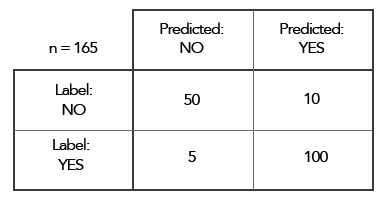
\includegraphics[scale=0.6]{confusion-matrix}
		\caption{Example of confusion matrix}
		\label{fig:mesh6}
	\end{figure}

	As it own name describes, the output of this type of metric consists of a matrix which shows a complete evaluation of the model. By definition, an entry $i,j$ of the matrix denotes the amount of observations that belong to group $i$ but are predicted as group $j$ \cite{Scikit-learn}. For example, considering a binary classification problem in which there are two classes, YES and NO, for a test set composed by 165 samples, the matrix included in figure \ref{fig:mesh6} is obtained. 
	
	There are four groups that can be extracted from this matrix: True positives, the samples that are predicted as YES and that is in fact their true label, True Negatives, those cases that were predicted as NO and they are originally labelled as NO, False Positives, in which the predicted label is YES but they are actually negative, and False Negatives, those in which the predicted label is NO when their original label is YES.
	
	This metric an the one explained before, accuracy, can be related by taking the diagonal of the matrix and computing the next operation:
	
	\[
	\ \ acc = \frac{TruePositives +\ FalseNegatives}{Total\ number\ of\ samples} = 
	\ \ \frac{100 +\ 50}{165} = 0.91
	\]
	
	When the classification task consists on more than two classes, a multiclass problem, a similar definition of the confusion matrix can be extended from the binary problem. Considering a certain observation $C_k$, the True positive part of the matrix is placed in the exact point where the column and the row of this certain observation are crossed, i.e, when the predicted label is equal to the true label. The False positives samples are placed along the column $C_k$ for all the rows $C_0, ..., C_{k-1}, C{k+1}, ..., C_n$ which refers to all the samples that have been misclassified with the class $C_k$. The False negatives are, however, all the samples that originally are labelled with $C_k$ tag but have been wrongly categorized with $C_0, ..., C_{k-1}, C{k+1}, ..., C_n$ classes. Finally, the True negative samples are distributed across all the other positions in the matrix. In figure \ref{fig:mesh9}, a good example for this explanation is shown.
	
	\begin{figure}[h]
		\centering
		\captionsetup{justification=centering}
		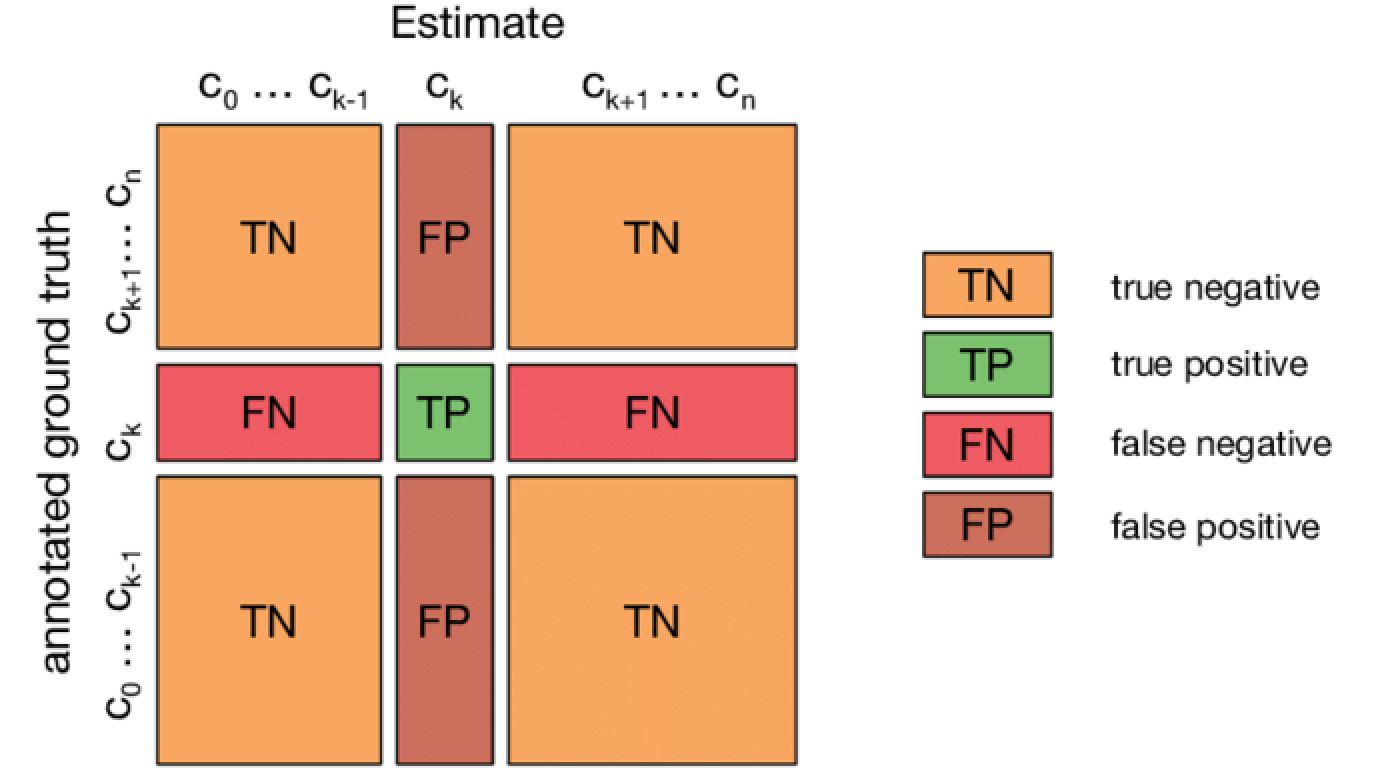
\includegraphics[scale=0.4]{conf-mat-multi}
		\caption{Confusion matrix for a multiclass classification \cite{Kruger2018}}
		\label{fig:mesh9}
	\end{figure}
	